\documentclass[../main.tex]{subfiles}
\graphicspath{{\subfix{../}}}
\begin{document}

\chapter{The IMF Language Implemented}
\label{ch:The IMF Language Formalized}

The IMF language is implemented using semantic web technologies. These artefacts are published at \url{http://ns.imfid.org}.

The IMF Ontology is defined by a Web Ontology Language (OWL) ontology, also called the IMF Ontology.
The ontology includes all the terms of the IMF language described with different metadata, including a textual definition, and their formal semantics which details how a term is related to other terms in the language. 
%
The grammar of the IMF language is specified by a set of SHACL shape specifications. They describe the required and permissible ways terms in the IMF Ontology may be used.
%

%The normative description of the IMF language is found in the OWL ontology and the SHACL shapes published at \url{http://ns.imfid.org}. 

%An informative extract from these artefacts is given in \autoref{ch:imf-ontology}. The formalisation of IMF types are presented in \autoref{ch:types}.


%\section{IMF Ontology}
\label{ch:imf-ontology}

%\input{chapters/M-imf-language-ontology}
%\section{IMF Types}
\label{ch:types}

An \emph{IMF type} is formally specified as a SHACL shape constraint
over the IMF language as defined by the IMF Ontology. The IMF type
SHACL shape should describe the required properties and values for
properties using the constructs available in the SHACL language. This
includes specifying, e.g., mandatory and optional properties,
fixed values, and value ranges.

A rudimentary grammar, (also) in the form of a SHACL shape constraint,
for IMF types is defined and made available at
\url{http://ns.imfid.org}. The grammar extends the standardised SHACL
shape specification published by W3C. The IMF type grammar specifies
three kinds of types: \texttt{BlockType}, \texttt{TerminalType} and
\texttt{AttributeType}. IMF types that follow the specified grammar
can be translated to an OWL class representation, and to
prototypical instance data following the IMF Ontology. The translation
tools are found from \url{http://ns.imfid.org}.

The OWL representation of an IMF type represents the class of instances
of the type, and instances of a type should explicitly be typed as
member of this class. The IMF SHACL shape for a type should use the
same IRI as for the OWL class.
%, but appended with
%\texttt{Shape}. Example: An IMF type for a pumping function could be
%represented by an \emph{SHACL shape} with IRI
%\texttt{ex:PumpingFunctionShape} and an \emph{OWL Class} with IRI
%\texttt{ex:PumpingFunction}. An instance of the type,
%e.g,. \texttt{abc:myPumpingFunction123}, should be explicitly be typed
%as member of the OWL class \texttt{ex:PumpingFunction} and it should
%validate against the SHACL shape \texttt{ex:PumpingFunctionShape}.

The OWL representation of a IMF type is useful for checking the
consistency of the type, to classify instances according to types, and
to discover specialisation/generalisation relationships between types
by reasoning over a set of types in OWL format and the IMF Ontology.

The prototypical type instance generated from an IMF type can be
useful as a starting point for specifying customised instances of the
type.

To simplify the creation of IMF types, a rudimentary tabular format
for specifying IMF types is defined using OTTR templates and
implemented as an annotated spreadsheet format.  \autoref{fig:Figure
  29} presents an overview of these OTTR templates.  The contents of
the spreadsheets in this format can be translated to SHACL shape
descriptions that follow the IMF type grammar. The OTTR templates are
available at \url{http://ns.imfid.org}. 

\begin{figure}[htb]
  \centering
  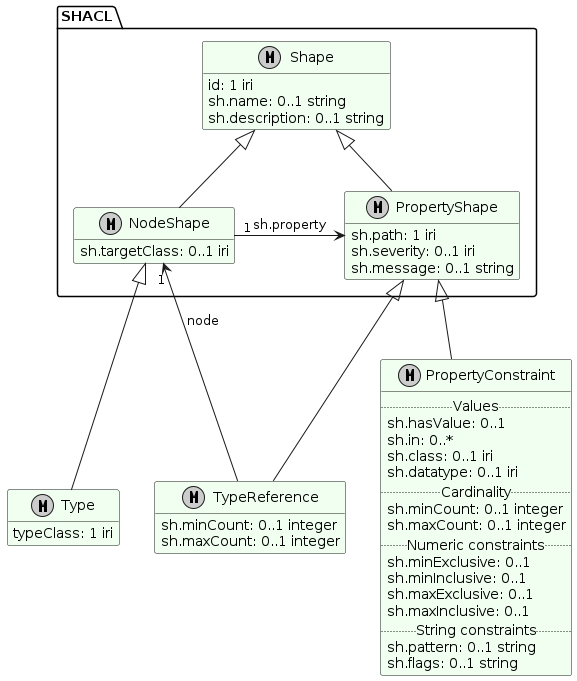
\includegraphics[width=.8\textwidth]{img/types/imf-types.png}
  \caption{IMF type OTTR Template patterns}
  \label{fig:Figure 29}
\end{figure}

An example that demonstrates the use of all the IMF semantic resources is
available from \url{http://ns.imfid.org}.





% An \emph{IMF type} (in this section also just called \emph{type}) is a construct from
% which IMF elements can be specified and created. The purpose of types is threefold:

% \begin{enumerate}
%   \item Standardization
%   \item Support reuse and avoid duplication of work
%   \item Classification
%   \end{enumerate}

% An element created from a type is called an \emph{instance}, and the operation of
% creating an instance by using a type is called \emph{instantiation}.
% An instance of a type must follow the pattern or requirements
% specified by the type, including attributes and relations. A type may
% specify both mandatory or optional requirements.

% An IMF type is implemented as a SHACL shape specification that
% specifies an RDF pattern over the IMF Ontology.  Instances of the
% pattern defined by the IMF type must respect the contraints set by the
% IMF Ontology and the SHACL shape that defines the IMF Model Grammar,
% including the requirements of the IMF type SHACL shape specification.

% There are currenly three kinds of types Block type, Terminal type, and
% Attribute type, which respectively specify a Block, a Terminal and an
% Attribute. A grammar for IMF types is specified as a SHACL shape
% description, available at \url{http://ns.imfid.org}.


% IMF types may again be translated to an OWL class representation of
% the type, and to a prototypical instance of the type. The translation
% is done using tools that can be found from \url{http://ns.imfid.org}.
% The OWL class representation of the IMF type specify the class of
% instances of the type.

% All IMF type SHACL shape specifications IRIs should end with the
% string \texttt{Shape}, and its OWL representation should be equal to
% the SHACL shape IRI but without the trailing \texttt{Shape}. For
% example, for a Pumping function type, the IRI of the SHACL Shape
% description could be \texttt{ex:PumpingFunctionShape}---then the IRI
% of its OWL representation must be \texttt{ex:PumpingFunction}.

% An instance of a type should be explictly be stated as member of the
% type's OWL class representation, e.g., a instance,
% \texttt{abc:myPumping}, is stated as an instance of the Pumping
% function with the following statement: \texttt{abc:myPumping rdf:type
%   ex:PumpingFunction}.











% Types are represented in the IMF framework as SHACL constraints on OWL classes that IMF elements are member of, expressed with the \texttt{rdf:type} property.


% All Types may specify an arbitrary set of classifiers whose values are typically resources from reference data
%   libraries (RDLs), i.e., reference data.

% An AttributeType is a type for Attributes. It should state a classifier that is the property of the
%   instantiating Attributes. Additionally, an AttributeType may state different constraints that constrain the
%   permissible values for an instantiating Attributes. 
%   The constraints themselves are not part of the pattern that instances of the Attribute type must follow,
%   i.e., the instantiating Attributes should not contain the constraints. A constraint may limit the permissible
%   values for an Attribute by specifying a list of legal values, legal datatype, and/or regular expression. Other
%   kinds of constraints may be possible depending on the implementation of types.

%   An ElementType is either a BlockType or a TerminalType. An ElementType may state a notation, which may be any value,
%   but typically a string, and a symbol that is used to visualize instances of the type. An ElementType may also state
%   an Aspect using the hasAspect relation. An ElementType specifies a set of attributes, via hasAttributeType
%   relationships to AttributeTypes, or via hasAttributeGroupType relationships to AttributeGroupTypes. These
%   relationships must be constrained by cardinality constraints that specify the minimum and maximum number of required
%   instances required of the related types. Optional attributes are specified for a type are specified by setting
%   minimum cardinality to 0. Mandatory attributes are specified by setting a number greater than 0.

% A TerminalType is an ElementType and is a type for Terminals. It may state a Medium and a Direction.

%  A BlockType is an ElementType and a type for Blocks. It may specify a set of Terminals, via hasTerminalType
%   relationships to TerminalTypes. The relationships must be constrained by cardinality constraints.

% instanceOf is a relation between an object and a type and expresses that the object is an instance of the type. This
%   statement is true if the object fulfills the constraints expressed for the type. This means that the object must
%   state all fields stated for the type, and that the object must state all the mandatory attributes stated for the type
%   and abide by the constraints stated on the AttributeTypes stated for the Type. 



% \paragraph{Discussion on different implementations of types}

% Types are meant to serve a range of purposes. This makes it relevant to implement the functionality of types with
% different languages.

% \begin{itemize}
%   \item A type may be represented as a (SHACL) constraints, where the instances of the type are objects that satisfy the
%         constraints. This implementation is useful for (automatically) verifying that the stated instances of a type follow
%         the requirements stated by the type.
        
%   \item A type can be represented as a \emph{prototypical} object.
%         Instances of the type are created from the type by ``copying the type'' and further detailing the copy according to
%         the constraints stated on the type.
        
%   \item A type can be represented as a (OWL) class, whose members are the instances of the type. A class implementation
%         is useful for classifying objects according to a set of types, and for identifying specialization/generalization
%         relationships between types.

%   \item A type may be represented as a (OTTR) template, where the instances of the type are created by instantiating the
%         template. This implementation is useful for easily creating type instances with a certain guarantee of correctness.
% \end{itemize}


\end{document}
